% Karrera Amarierako Proiektua egiteko LaTeX txantiloia
% itsas.ehu.es/workgroups/latex
% Unai Martinez Corral
% umartinez012@ikasle.ehu.es
%
% <- sectb_main.tex

\titlesubsection{Liburutegiak}

VHDL-93 estandarreko \emph{numeric\_std} paketearen \emph{shift\_right}, \emph{shift\_left} eta \emph{resize} funtzioen argibideak jarraituz, hauek dira informazio esanguratsua babestuz koma bitarraren kokapenaren araberako moldaketak burutzeko erabilitako adierazpenak:

\begin{description}
\item[resize(shift\_right(\emph{signal},$n$),$wl-n$)]{\hfill \\Pisu gutxieneko bitak galduz seinalea moztea}
\item[shift\_right(\emph{signal},$n$)]{\hfill \\Luzera mantenduz koma bitarra eskumara mugitzea edo $2^{n}$ aldiz zatitzea}
\item[shift\_left(resize(\emph{signal},$wl+n$),$n$)]{\hfill \\Koma hitza luzatuz ezkerrera mugitzea edo $2^{n}$ aldiz biderkatzea}
\end{description}

Laburbilduz, \emph{IEEE} liburutegiko \emph{sdt\_logic\_1164} eta \emph{numeric\_std} paketeak baino ez dira kargatu. Burutuko ditugun eragiketak oso konplexuak ez direnez sintetizatzean programak berak aukeratuko ditu, \emph{IP Core} bereziren instantzia barik. Hauen beharra kodearen bitartez adieraziko dugu, modu funtzionalean.

\lstinputlisting[firstline=4,lastline=6]{anie_vhdl_pid.vhd}

\titlesubsection{Entitatea}

\lstinputlisting[firstnumber=last,firstline=9,lastline=9]{anie_vhdl_pid.vhd}

\subsubsection{\emph{generic} parametroak}

Kontroladorearen erabilera errazteko, eta konfigurazio denbora murrizteko, seinale guztiak parametrizatu egin dira. Honela, aldagaien ($i\_wl$), irteeraren ($o\_wl$), koefizienteen ($k\_wl$) edota funtzio integratzailearen memoriaren ($irem\_wl$\footnote{$irem\_wl$-ren funtsa \emph{anti-windup} estrategiaren deskribapenean azaltzen da.}) hitz luzera aldatuz gero barne egitura moldatzen da.

\subsubsection{Atakak}

\lstinputlisting[firstnumber=last,firstline=21,lastline=30]{anie_vhdl_pid.vhd}

\titlesubsection{Arkitektura}

\subsubsection{Osagaiak}

Sarrerekin gertatu bezala, VHDL deskribapenean kontroladoreak aurreko modeloetan irteeran agertu izan den saturazio blokea ere barnean izango du. Adar integratzailean ere, \emph{windup} arazoa konpontzeko erabilitako estrategiaren arabera, saturatzeko beharra izan dezakegu. Horregatik sarreran seinale bat jaso eta irteeran saturatutako seinale berdina ateratzen duen parametrizatutako osagaia deskribatu da.

\noindent
\begin{minipage}{.45\textwidth}
\lstinputlisting[firstnumber=last,firstline=33,lastline=38]{anie_vhdl_sat.vhd}
\end{minipage}
\hspace{.5em}
\begin{minipage}{.5\textwidth}
\centering
% Karrera Amarierako Proiektua egiteko LaTeX txantiloia
% itsas.ehu.es/workgroups/latex
% Unai Martinez Corral
% umartinez012@ikasle.ehu.es
%
% <- sectb_first.tex

\tikzstyle{un} = [draw, circle, fill=black!75!blue]
\tikzstyle{resize} = [draw, rectangle,\const, fill=blue!30]
\tikzstyle{inout} = [rectangle]
\tikzstyle{block} = [draw, rectangle, minimum height=2.5em, minimum width=3.5em]
\tikzstyle{cblock} = [draw, rectangle, minimum height=2.5em, minimum width=2.25em]

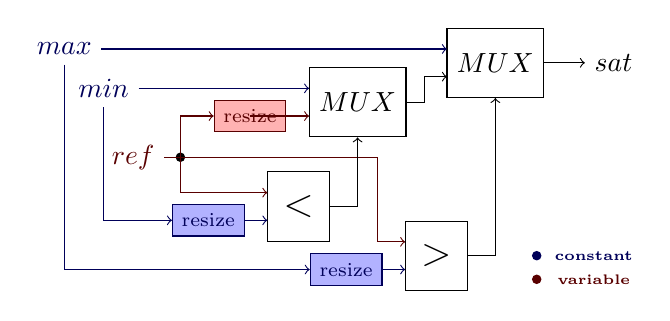
\begin{tikzpicture}[auto,node distance=1cm]
  \def\sep{1cm}
  \def\bh{.5em}
  \def\bw{1.75em}
  \def\bwc{1.125em}
  \def\const{black!65!blue}
  \def\var{black!65!red}

  \node [inout,\const] (max) {$max$};
  \node [coordinate, below of=max, node distance=.5*\sep] (max_r_b) {};

  \node [inout, \const,right of=max_r_b, node distance=.5*\sep] (min) {$min$};
  \node [coordinate, right of=min, node distance=.375*\sep] (min_r) {};

  \node [inout, \var, below of=min_r,node distance=.875*\sep] (ref) {$ref$};
  \node [coordinate, right of=ref, node distance=.6*\sep] (ref_r) {};
  \node [coordinate, right of=ref_r, node distance=1.5*\sep] (cn_p) {};

  \node [cblock, below of=cn_p,node distance=.625*\sep] (cn) {\Large $<$};
  \node [coordinate, left of=cn,node distance=\bwc] (cnw) {};
  \node [coordinate, above of=cnw,node distance=\bh] (cnwa) {};
  \node [coordinate, below of=cnw,node distance=\bh] (cnwb) {};
  \node [coordinate, right of=cn,node distance=.75*\sep] (cn_r) {};
  \node [coordinate, right of=cn_r,node distance=.25*\sep] (cn_r_r) {};

  \node [resize,left of=cnwb,node distance=.75*\sep] (nres) {\scriptsize resize};

  \node [coordinate, right of=cn_p,node distance=.75*\sep] (mn_p) {};
  \node [block, above of=mn_p,node distance=.875*\sep-\bh] (mn) {$MUX$};
  \node [coordinate, left of=mn,node distance=\bw] (mnw) {};
  \node [coordinate, above of=mnw,node distance=\bh] (mnwa) {};
  \node [coordinate, below of=mnw,node distance=\bh] (mnwb) {};
  \node [coordinate, right of=mn,node distance=.85*\sep] (mn_r) {};

  \node [resize,\var,fill=red!30,left of=mnwb,node distance=.75*\sep] (rres) {\scriptsize resize};

  \node [coordinate, below of=cn,node distance=.75\sep] (cn_b) {};

  \node [coordinate, right of=mn_p,node distance=\sep] (cm_p) {};
  \node [cblock, below of=cm_p,node distance=1.25*\sep] (cm) {\Large $>$};
  \node [coordinate, left of=cm,node distance=\bwc] (cmw) {};
  \node [coordinate, above of=cmw,node distance=\bh] (cmwa) {};
  \node [coordinate, below of=cmw,node distance=\bh] (cmwb) {};
  \node [coordinate, right of=cm,node distance=.75*\sep] (cm_r) {};

  \node [resize,left of=cmwb,node distance=.75*\sep] (pres) {\scriptsize resize};

  \node [block, above of=cm_r,node distance=2.625*\sep-\bh] (mm) {$MUX$};
  \node [coordinate, left of=mm,node distance=\bw] (mmw) {};
  \node [coordinate, above of=mmw,node distance=\bh] (mmwa) {};
  \node [coordinate, below of=mmw,node distance=\bh] (mmwb) {};

  \node [inout, right of=mm,node distance=1.5*\sep] (sat) {$sat$};

  \node [inout,\const,right of=cm_r, node distance=1.25*\sep] (constant) {\tiny \textbf{constant}};
  \node [inout,\var,below of=constant, node distance=.3*\sep] (variable) {\tiny \textbf{variable}};
  \node [coordinate,\const,left of=constant,node distance=.725*\sep] (constlg) {};
  \node [coordinate,\var,left of=variable,node distance=.725*\sep] (varlg) {};
  \draw[fill,\const](constlg) circle (1.5pt);  
  \draw[fill,\var](varlg) circle (1.5pt);

  \draw[fill](ref_r) circle (1.5pt);

  \draw [->,\var] (ref_r) |- (cnwa);
  \draw [->,\const] (nres) -- (cnwb);
  \draw [->,\const](min) |- (nres);

  \draw [->,\var] (ref) -| (cn_r_r) |- (cmwa);
  \draw [->,\const] (pres) -- (cmwb);
  \draw [->,\const] (max) |- (pres);

  \draw [->] (cn) -- (cn_r) -- (mn);
  \draw [->] (cm) -- (cm_r) -- (mm);

  \draw [->,\const] (min) -- (mnwa);
  \draw [->,\var] (rres) |- (mnwb);
  \draw [->,\var] (ref_r) |- (rres);

  \draw [->,\const] (max) -- (mmwa);
  \draw [->] (mn.east) -- (mn_r) |- (mmwb);

  \draw [->] (mm) -- (sat);
\end{tikzpicture}

\end{minipage}

\subsubsection{Seinaleak}

\begin{table}[!htp]
\centering
\begin{tabular}{ccc|ccc}
\textbf{id} & \textbf{msb} & \textbf{comment} & $\quad$ \textbf{id} & \textbf{msb} & \textbf{comment}\\
\hline
\hline
&&&&&\\
$ref$ & \multirow{2}{*}{i\_wl-1} & $r(k)\quad$ & $\quad int_{mult}$ & \multirow{2}{*}{mw} & $K_i \cdot (e(k) + e(k-1))$ \\
$feed$ & & $y(k)\quad$ & $\quad der_{out}$ & & $K_d \cdot (e(k) - e(k-1))$ \\
&&&&&\\
$dif_{act}$ & \multirow{2}{*}{aswl-1} & $e(k)\quad$ & $\quad int_{out}$ & \multirow{3}{*}{oswl-1} & $u_{isat}(k)$ \\
$dif_{pre}$ & & $e(k-1)\quad$ & $\quad int_{rem}$ & & $u_{isat}(k-1)$ \\
&&& $\quad out_{sat}$ & & $u_{sat}(k)$ \\
$int_{sum}$ & \multirow{2}{*}{aswl} & $e(k) + e(k-1)\quad$ &&& \\
$der_{dif}$ & & $e(k) - e(k-1)\quad$ & $\quad int_{tosat}$ & \multirow{2}{*}{oswl} & $u_{i}(k)$ \\
&&&$\quad out_{tosat}$ & & $\quad u(k)$ \\
$pro_{out}$ & mwl-1	& $K_p \cdot e(k)\quad$ &&&\\
\end{tabular}

\begin{minipage}{.55\textwidth} \begin{lstlisting}
 signal id: signed(msb downto 0); --comment
\end{lstlisting} \end{minipage}
\caption{Kontroladorearen arkitekturan deklaratutako seinaleak eta hitz luzerak.}
\label{tab:vhdl_signals}
\end{table}
